%!TEX root = ../../Master.tex
\section{Triangulation}

\subsection{Lateration}

  \begin{figure}[ht!]
  \centering
  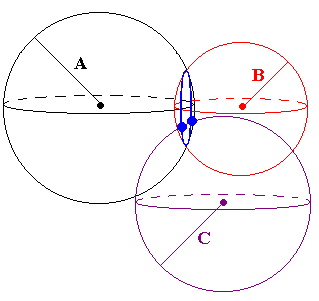
\includegraphics[width=3in]{trilateration}
  \caption{Example of lateration with three know positions.}
  \label{fig:trilateration}
  \end{figure}
  

  Trilateration in three dimensions is possible in fare most situations if and only if the distance to three known positions is defined or possible to calculate.
  If we know a distance to one of these three positions we know that the point we are seeking is in the surface of a sphere, with center at the know position, and with a radius equals to the distance to the center. This is illustrated on \cref{fig:trilateration} as the surface of the sphere A.

  The intersection of two spheres is a circle. By determining the distance to a second know point it is possible to circumscribe the range of possible position to a smaller area.
  This is illustrated as the blue circle on \cref{fig:trilateration}, and is the intersection between sphere A and B.
  A third sphere that overlaps the intersection between the first two spheres, will mark 2 points where all three spheres is collapsing. In fare most situations there are only one of these locations that lies on the Earth's surface, the other point will often be fare in to the sky or deep inside earth. So by sorting one point from, there is only one possible position left. 
  In some very rare situation it is possible that both point lies on the Earth's surface, and in such situations the use of four spheres will determine witch of the to positions is the right one.



\subsection{Angulation}


	\sinote{Needs introduction}

  For example, rangers in location known fire lookout towers can use AOA to pinpoint where the fire is. See \cref{fig:aoa} A ranger at tower A sees the fire and notates the bearing to the fire. He then communicates with a ranger at tower B telling him the general direction of the fire. The ranger at tower B now notates the bearing to the fire from his perspective. The fire can now be pinpointed from the 2 remote points (given the fire started in a 2-D world). The fire is where the 2 angle direction lines intercept A ranger at tower C can verify this position by also noting his bearing. \cite{compassdude_triangulation}

  \begin{figure}
    \centering
    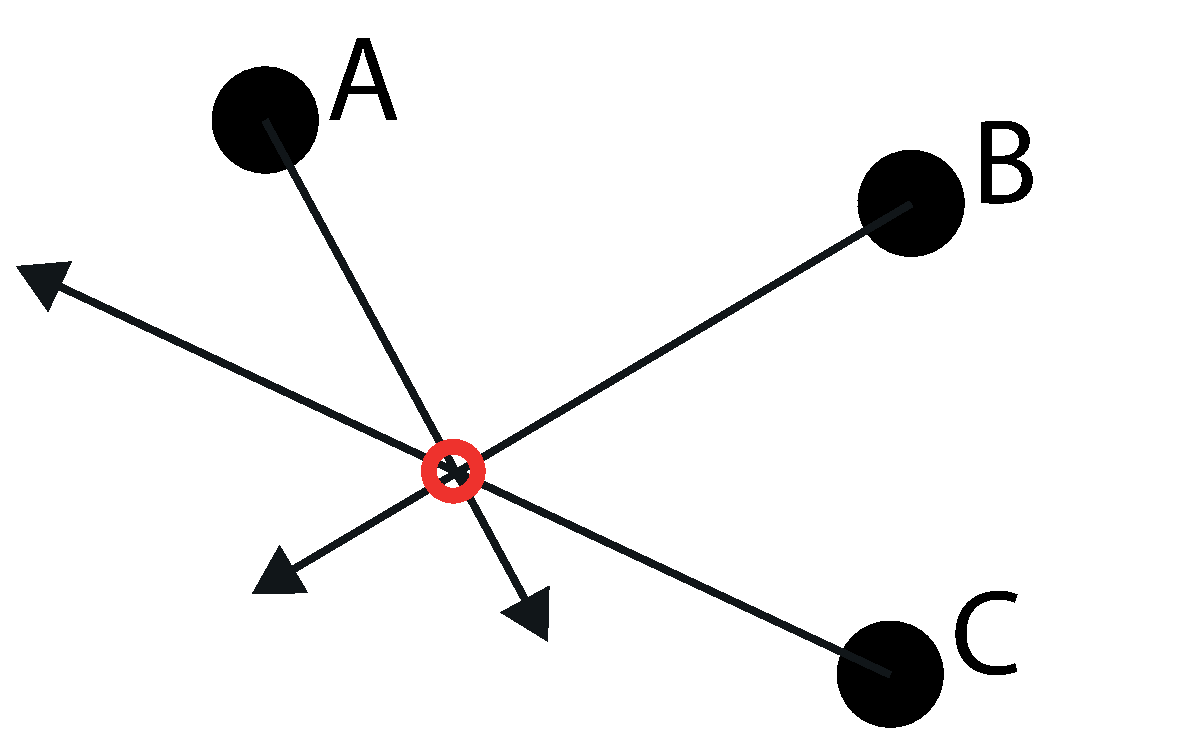
\includegraphics[width=0.5\textwidth]{aoa.eps}
    \caption{Example of fire lookout towers positioning a fire using AOA.}
      \label{fig:aoa}
  \end{figure}

  The advantages of AOA are the few remote points needed in order to estimate a position. Another advantage is the independency of time synchronization.

  The disadvantages of AOA are the need of large and complex hardware requirements, and degradation of the location estimate as the target moves away from the measuring units. In order to perform accurate position of the target, very accurate angle measurements need to be performed. This can become a problem if the measuring is done in wireless networks, because of shadowing, multipath reflections arriving from misleading directions etc. Therefore angulation is best performed in free space.